\section{Experiments}\label{sec:experiments}
\subsection{Questions and protocol}
The experiments test the consequences of the exact local identity and the
search procedure derived from it. We ask: (Q1) how often do established
constructors leave an improving NNI;
(Q2) does compound search add improvements beyond a one-step certificate;
(Q3) does lower entropy preserve or improve recovery of a planted hierarchy;
and (Q4) how close is \NEST to the global optimum on exactly solvable graphs?

The sealed main protocol uses 100 graph seeds per regime. Every method sees the
identical weighted graph, every tree is rescored by the same independent
implementation of Eq.~\eqref{eq:tree-se}, and we report paired means with 95\%
$t$-intervals. The compound search uses beam width 16, barrier $\beta=0.05$ bits, and at
most eight accepted compound rounds. No label is used by \NEST for model
selection. BBM is additionally shown with the planted number of fine clusters,
which is an oracle advantage and is marked as such.

\paragraph{Data.}
Our controlled suite contains five two-level hierarchical stochastic block
models: clean, noisy, imbalanced, weighted, and weak-hierarchy. Each balanced
graph has 64 vertices, eight fine blocks, and four coarse blocks; the
imbalanced regime has the same total size with block sizes from 4 to 12. The
generator manifest, any $0.01$-weight connectivity edges, and every seed are
stored with the results. This family follows the hierarchical stochastic block
model used to study recovery beyond worst-case inputs \cite{cohenaddad2017hsbm}.

\paragraph{Methods.}
We compare SE agglomeration, a two-level Louvain tree \cite{blondel2008}, Paris
\cite{bonald2018paris}, official HCSE, official BBM with oracle $k$
\cite{pan2025}, and \NEST, whose pool (SE agglomeration, recursive SE, Paris)
excludes HCSE, BBM, and Louvain-2L; these remain external comparators. The
operator audit separately applies NNI to every constructor's returned tree.

\paragraph{Metrics.}
The primary metric is $\HT(G)$. Dendrogram purity is computed for the planted
fine and coarse partitions: for every same-class vertex pair, it measures the
class fraction under the pair's predicted LCA, then averages over pairs. For
the exact suite we report the relative gap
$100(H^T_{\rm NEST}-H^*)/H^*$ and the \emph{optimal-hit rate}: the fraction of
graphs whose objective is within $\max(10^{-9},10^{-8}|H^*|)$ of the exact
optimum.

\subsection{Frozen benchmark results}
\emph{{\upshape\NEST} returns the lowest-entropy tree on every one of the 500 graphs.}
Table~\ref{tab:main-h} compares the tree returned by each standalone baseline
with the best verified endpoint of \NEST's three-initializer pool; the \NEST
row does not post-process HCSE or BBM outputs. \NEST has the lowest mean $\HT$
in all five regimes. Relative to HCSE and BBM, its paired reductions are
$\NESTGainVsHCSE\!\pm\!\NESTGainVsHCSECI$ and
$\NESTGainVsBBM\!\pm\!\NESTGainVsBBMCI$ bits. Figure~\ref{fig:entropy} plots,
for each graph $g$, the margin
$M_g=\min(H^T_{\mathrm{HCSE},g},H^T_{\mathrm{BBM},g})-H^T_{\mathrm{NEST},g}$
against the stronger baseline; all 500 margins are positive. BBM's internal
clustering is unseeded: rerunning 15 of these graphs changed its entropy by at
most 0.10 bits, below the smallest margin of 0.19 bits. \NEST, HCSE, Paris,
and both SE constructors reproduced bit-for-bit.

\begin{table}[t]
\centering\small
\caption{Mean tree structural entropy $H^T$ (bits) on 100 paired graphs per
HSBM regime. The $\pm$ value is a 95\% $t$-interval over graph seeds; lower is
better, and bold marks the lowest column mean. BBM$^\dagger$ receives the
planted fine-cluster count; the other methods do not use labels.}
\label{tab:main-h}
\setlength{\tabcolsep}{0pt}
\begin{tabular*}{\textwidth}{@{\extracolsep{\fill}}lccccc@{}}
\toprule
Method & Clean & Noisy & Imbalanced & Weighted & \shortstack{Weak\\hierarchy} \\
\midrule
SE--agglomerative & 2.899\,{\scriptsize$\pm$0.021} & 3.723\,{\scriptsize$\pm$0.017} & 3.162\,{\scriptsize$\pm$0.023} & 2.445\,{\scriptsize$\pm$0.016} & 3.461\,{\scriptsize$\pm$0.022} \\
Louvain--2L & 4.109\,{\scriptsize$\pm$0.022} & 4.603\,{\scriptsize$\pm$0.013} & 4.241\,{\scriptsize$\pm$0.019} & 3.657\,{\scriptsize$\pm$0.032} & 4.432\,{\scriptsize$\pm$0.018} \\
Paris & 2.869\,{\scriptsize$\pm$0.022} & 3.709\,{\scriptsize$\pm$0.017} & 3.129\,{\scriptsize$\pm$0.023} & 2.349\,{\scriptsize$\pm$0.015} & 3.438\,{\scriptsize$\pm$0.023} \\
HCSE & 3.228\,{\scriptsize$\pm$0.031} & 4.485\,{\scriptsize$\pm$0.068} & 3.598\,{\scriptsize$\pm$0.036} & 2.741\,{\scriptsize$\pm$0.029} & 4.032\,{\scriptsize$\pm$0.051} \\
BBM$^\dagger$ & 3.335\,{\scriptsize$\pm$0.021} & 4.118\,{\scriptsize$\pm$0.020} & 3.573\,{\scriptsize$\pm$0.025} & 3.007\,{\scriptsize$\pm$0.020} & 3.924\,{\scriptsize$\pm$0.022} \\
\midrule
\NEST\ (ours) & \textbf{2.827\,{\scriptsize$\pm$0.021}} & \textbf{3.683\,{\scriptsize$\pm$0.017}} & \textbf{3.086\,{\scriptsize$\pm$0.023}} & \textbf{2.340\,{\scriptsize$\pm$0.015}} & \textbf{3.414\,{\scriptsize$\pm$0.021}} \\
\bottomrule
\end{tabular*}
\end{table}


\begin{figure}[t]
  \centering
  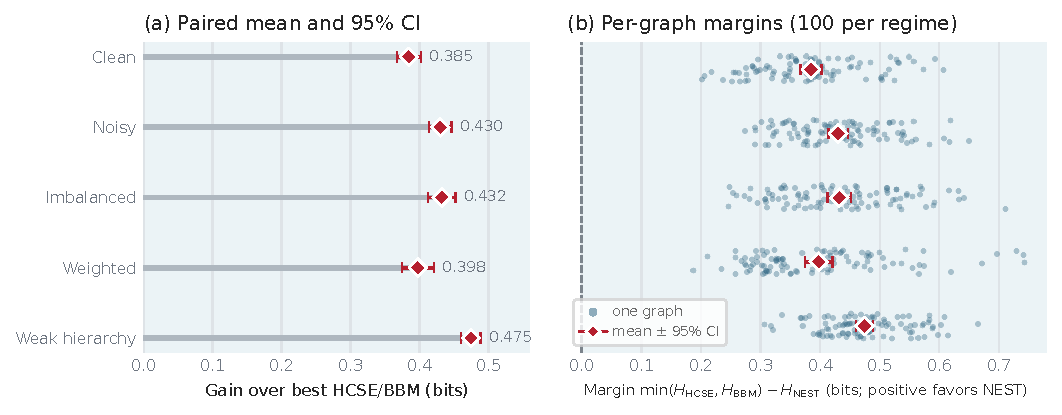
\includegraphics[width=\textwidth]{figures/benchmark_entropy.pdf}
  \caption{Paired advantage over external structural-entropy methods. For graph
  $g$, the margin is
  $M_g=\min(H^T_{\mathrm{HCSE},g},H^T_{\mathrm{BBM},g})-H^T_{\mathrm{NEST},g}$,
  so positive values favor \NEST. (a) Regime mean and paired 95\% confidence
  interval. (b) Each blue dot is one of 100 sealed graphs per regime; vertical
  jitter only separates overlapping dots. Red diamonds are regime means and
  horizontal whiskers are their 95\% confidence intervals. All 500 margins are
  positive.}
  \label{fig:entropy}
\end{figure}

\emph{Lower entropy coincides with better planted-hierarchy recovery on
average, but not on every graph} (Q3). Fine-level dendrogram purity is
\PurityFineNEST{} for \NEST, versus \PurityFineHCSE{} for HCSE and
\PurityFineBBM{} for oracle-$k$ BBM; the paired gains are
$\PurityFineGainHCSE\!\pm\!\PurityFineGainHCSECI$ and
$\PurityFineGainBBM\!\pm\!\PurityFineGainBBMCI$. Coarse-level gains are
$\PurityCoarseGainHCSE\!\pm\!\PurityCoarseGainHCSECI$ and
$\PurityCoarseGainBBM\!\pm\!\PurityCoarseGainBBMCI$. \NEST's fine purity is
nonetheless lower than HCSE's on \PurityFineLowerHCSE{} graphs, so entropy is
not a proxy for recovery on an individual instance.

\subsection{The operator audit}
\emph{Constructor quality and NNI-local optimality are different properties}
(Q1, Q2). Table~\ref{tab:operator} applies the same
two-stage refinement to each constructor's output: one-NNI descent commits the
best decreasing move until none remains, and the two-move escape then accepts
only a lower-entropy endpoint of a bounded pair. One-step NNI improves every
SE-agglomerative and oracle-BBM tree, and after that certificate the two-move
escape still improves 62\% and 93\% of them. On \BBMBudgetHits{} BBM trees
descent reached the $M=100$ move budget, so the BBM drops are lower bounds. Paris trees are improved in 74\%
and then 41\% of graphs. HCSE trees are nearly NNI-locally optimal, with rates
of 3\% and 4\%, yet their mean entropy exceeds that of Paris in every regime of
Table~\ref{tab:main-h}.

\begin{table}[t]
\centering\small
\caption{NNI refinement audit over 500 graphs. Drop is mean reduction relative
to raw $H^T$; improved is the fraction of graphs with a strict reduction.
Two-move values are additional to one-NNI descent, and time excludes initial
tree construction.}
\label{tab:operator}
\begin{tabular*}{\textwidth}{@{\extracolsep{\fill}}lccccc@{}}
\toprule
& \multicolumn{2}{c}{One-NNI descent}
& \multicolumn{2}{c}{Two-move escape}
& \shortstack{Refinement\\time} \\
\cmidrule(lr){2-3}\cmidrule(lr){4-5}
Constructor
& \shortstack{Entropy\\drop}
& \shortstack{Graphs\\improved}
& \shortstack{Extra entropy\\drop}
& \shortstack{Graphs further\\improved}
& (s) \\
\midrule
SE--agglomerative & 1.97\% & 100\% & 0.14\% & 62\% & 0.642 \\
Paris & 0.07\% & 74\% & 0.06\% & 41\% & 0.388 \\
HCSE & 0.00\% & 3\% & 0.00\% & 4\% & 0.108 \\
BBM$^\dagger$ & 14.02\% & 100\% & 0.46\% & 93\% & 1.962 \\
\bottomrule
\end{tabular*}
\end{table}




\subsection{Components and exact optimality}
\emph{Every component of {\upshape\NEST} contributes.} On a separate frozen 50-graph
subset (full ablation table in \ablationdetails), starting from SE agglomeration, the
candidate pool improves 34 graphs, one-NNI descent then improves 45, and the
two-move escape adds gains on 30. The main benchmark's verifier checks hashes,
schema, paired seeds, unique keys, and monotonicity of committed NNI endpoints
across its 3,500 method records and 500 generator manifests.


\emph{On exactly solvable graphs, 32 coalescent starts reach the global optimum
in \ScaleCombinedExact{} cases} (Q4). Disjoint calibration fixed $q=32$; we
then sealed 250 graphs at $n=12$, 100 at $n=14$, and 25 at $n=16$ across the
same five regimes. Every method receives exactly 32 candidates: coalescent
starts for \NEST; eight seeded HCSE calls at each target height 2--5; and
label-free BBM calls cycling through $k=2,\dots,8$ (four or five per $k$). The
deterministic \NEST pool is excluded from this budget. HCSE is nearly
deterministic, returning at most \HCSEMaxDistinct{} distinct entropies per
graph, whereas BBM returns \BBMDistinctRange{}. Selection uses only structural entropy, and the
exact dynamic program is consulted afterward. Table~\ref{tab:exact-scale}
reports 2/375 exact hits for HCSE and 1/375 for label-free BBM, with exact
binomial intervals for \NEST at each size. The interval widens to
[68.78, 97.45]\% at $n=16$, where only 25 graphs were audited. Every block has
status zero, matching SHA-256 seals, complete seed coverage, and independently
recomputed summaries; a fresh rerun of 15 of these graphs reproduced every
$H^*$ and every \NEST outcome.

\begin{table}[t]
\centering\small
\caption{Sealed exact-optimum audit on independently generated HSBMs with $n$
vertices and 32 candidates per method: coalescent starts for \NEST, target
heights for HCSE, and label-free cluster counts for BBM. Exact columns report
optimum hits over the listed graphs. The \NEST interval is an exact 95\% Clopper--Pearson
interval for its hit rate. Its relative gap is
$100(H^T_{\mathrm{NEST}}-H^*)/H^*$, reported as mean/worst; zero is optimal.
Candidate selection does not use $H^*$.}
\label{tab:exact-scale}
\begin{tabular*}{\textwidth}{@{\extracolsep{\fill}}rrccccc@{}}
\toprule
& & \multicolumn{3}{c}{Exact optima found}
& \multicolumn{2}{c}{\NEST diagnostics} \\
\cmidrule(lr){3-5}\cmidrule(lr){6-7}
$n$ & Graphs & \NEST & HCSE & BBM
& \shortstack{95\% hit-rate\\interval}
& \shortstack{Mean / worst\\relative gap} \\
\midrule
12 & 250 & \textbf{249/250} & 2/250 & 1/250 & [97.79, 99.99]\% & 0.00032\% / 0.07990\% \\
14 & 100 & \textbf{99/100} & 0/100 & 0/100 & [94.55, 99.97]\% & 0.00121\% / 0.12060\% \\
16 & 25 & \textbf{22/25} & 0/25 & 0/25 & [68.78, 97.45]\% & 0.03990\% / 0.44934\% \\
\bottomrule
\end{tabular*}
\end{table}


\subsection{Real networks}
\emph{{\upshape\NEST} also attains the lowest entropy on \RealWins{} real networks}
(Table~\ref{tab:real}). These networks lack a unique ground-truth hierarchy,
so this experiment measures objective minimization only. Paris is the closest
competitor, 0.004--0.019 bits behind.

\begin{table}[t]
\centering\small
\caption{Tree structural entropy $H^T$ (bits; lower is better) on four real
networks: Zachary karate club, Florentine families, Les Mis\'erables, and
Davis Southern women. Bold marks the lowest value per network.
BBM$^\dagger$ uses ground-truth $k$ for Karate and Louvain's $k$ otherwise.}
\label{tab:real}
\begin{tabular*}{0.90\textwidth}{@{\extracolsep{\fill}}lrrrr@{}}
\toprule
Method & Karate & Florent. & Les Mis. & Davis \\
\midrule
SE--agglomerative & 2.698 & 1.923 & 3.078 & 3.055 \\
Louvain--2L & 3.405 & 2.452 & 3.923 & 3.813 \\
Paris & 2.597 & 1.923 & 2.920 & 2.981 \\
HCSE & 2.929 & 2.172 & 3.930 & 3.206 \\
BBM$^\dagger$ & 3.330 & 2.254 & 3.199 & 3.387 \\
\midrule
\NEST\ (ours) & \textbf{2.586} & \textbf{1.919} & \textbf{2.916} & \textbf{2.962} \\
\bottomrule
\end{tabular*}
\end{table}

